\documentclass{article}

\title{Mini-project: Evil Toddlers and Stone Fruit}
\author{Henry Oehlrich \and Joe Coimbatore \and Noah Curtis}

\usepackage[margin=1.25in]{geometry}
\usepackage{pgfplots}
\usepackage{pgfplotstable}
\usepackage{pgf-pie}
\usepackage{caption}
\usepackage{subcaption}
\usepackage{booktabs}

\pgfplotsset{compat=1.8}
\pgfplotstableread[row sep=\\,col sep=&]{
    Do you know what a stone fruit is? & Number of evil toddlers \\
    Yes & 5.857 \\
    No & 23.304 \\
}\fruitandtoddlers
\captionsetup[figure]{labelfont={bf}}

\begin{document}
\maketitle
\begin{figure}
    \centering
    \caption{Data}
    \label{fig:data}
    \begin{subfigure}{.5\textwidth}
        \centering
        \label{fig:original}
        \caption{Original Data}
        \begin{tabular}{p{3cm}|p{3cm}}
            \toprule
            Know stone fruit? & \# evil toddlers \\
            \midrule
            No & 10 \\
            Yes & 20 \\
            No & 20 \\
            Yes & 5 \\
            Yes & maaaaaybe 2 \\
            No & 1 \\
            No & 20 \\
            No & 1 \\
            No & 100 \\
            No & 0 \\
            No & 100 \\
            No & 2 \\
            No & 2 \\
            No \\
            Yes & 0 \\
            No & 500 \\
            Yes & 5 \\
            No & 10 \\
            No & 2 \\
            No & 3 \\
            No & 100 \\
            No & 30 \\
            No & 3 \\
            No & 15 \\
            No & haven't tested it \\
            Yes & 2 \\
            No & 0 tbh (I'm a pacifist) \\
            No & 0 \\
            Yes & 7 \\
            No & 10 \\
            No & I might not be sure on that \\
            No & 4 \\
            No & 1000 \\
            No & 83 \\
            No & 20 \\
        \end{tabular}
    \end{subfigure}%
    \begin{subfigure}{.5\textwidth}
        \centering
        \label{fig:original}
        \caption{Modified Data}
        \begin{tabular}{p{3cm}|p{3cm}}
            \toprule
            Know stone fruit? & \# evil toddlers \\
            \midrule
            No & 10 \\
            Yes & 20 \\
            No & 20 \\
            Yes & 5 \\
            No & 1 \\
            No & 20 \\
            No & 1 \\
            No & 100 \\
            No & 0 \\
            No & 100 \\
            No & 2 \\
            No & 2 \\
            Yes & 0 \\
            Yes & 5 \\
            No & 10 \\
            No & 2 \\
            No & 3 \\
            No & 100 \\
            No & 30 \\
            No & 3 \\
            No & 15 \\
            Yes & 2 \\
            No & 0 \\
            No & 0 \\
            Yes & 7 \\
            No & 10 \\
            No & 4 \\
            No & 83 \\
            No & 20 \\
        \end{tabular}
    \end{subfigure}%
\end{figure}
\begin{figure}
    \centering
    \caption{Number of evil toddlers by knowledge of stone fruits}
    \label{fig:fruitandtoddlers}
    \begin{tikzpicture}
        \begin{axis}[
                width=1\textwidth,
                height=.5\textwidth,
                ymin=0,
                ymax=30,
                ylabel={Number of evil toddlers},
                xtick=data,
                xticklabels from table={\fruitandtoddlers}{Do you know what a stone fruit is?},
                xlabel={Do you know what a stone fruit is?},
                ybar,
                bar width=-.5,
                ybar=1pt,
                enlarge x limits={abs=0.5},
            ]
            \addplot table [x expr=\coordindex, y=Number of evil toddlers]{\fruitandtoddlers};
        \end{axis}
    \end{tikzpicture}
\end{figure}
\begin{figure}
    \centering
    \caption{How many evil toddlers could you beat in a fight?}
    \label{fig:toddlers}
    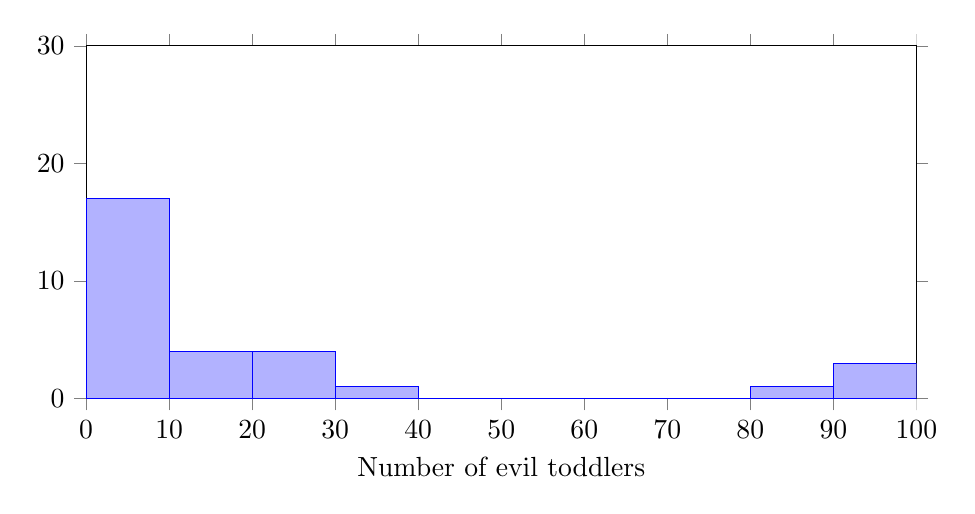
\begin{tikzpicture}
        \begin{axis}[
                width=1\textwidth,
                height=.5\textwidth,
                ymin=0,
                ymax=30,
                xlabel={Number of evil toddlers},
                xmin=0,
                xmax=100,
                xtick=data,
                ybar,
                tick align=outside,
            ]
            \addplot+[hist={bins=10}]
            table [row sep=\\,y index=0] {
                data\\
                10\\ 20\\ 20\\ 5\\ 2\\ 1\\ 20\\ 1\\ 100\\ 0\\ 100\\ 2\\ 2\\
                0\\ 5\\ 10\\ 2\\ 3\\ 100\\ 30\\ 3\\ 15\\ 2\\ 0\\ 0\\ 7\\
                10\\ 4\\ 83\\ 20\\
            };
        \end{axis}
    \end{tikzpicture}
\end{figure}
\begin{figure}
    \centering
    \caption{Do you know what a stone fruit is?}
    \label{fig:stonefruit}
    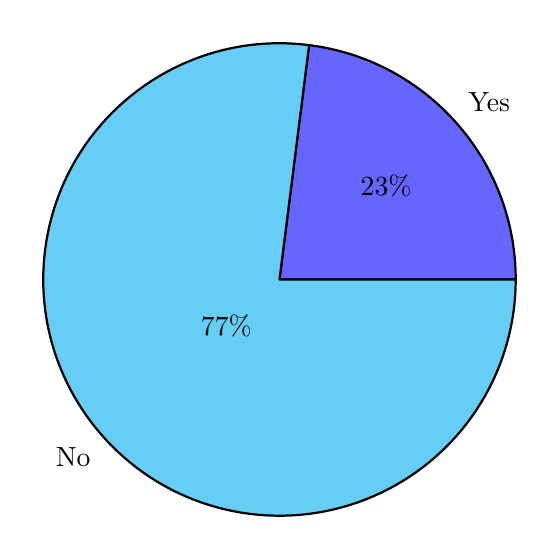
\begin{tikzpicture}
        \pie{23/Yes, 77/No}
    \end{tikzpicture}
\end{figure}
\end{document}
